\documentclass[dvipdfmx]{jsarticle}

\title{西暦和暦変換プログラムの作成(Java版)}
\author{Seiichi Nukayama}
\date{2020-05-05}
\usepackage{tcolorbox}
\usepackage{color}
\usepackage{listings, plistings}

% Java
\lstset{% 
  frame=single,
  backgroundcolor={\color[gray]{.9}},
  stringstyle={\ttfamily \color[rgb]{0,0,1}},
  commentstyle={\itshape \color[cmyk]{1,0,1,0}},
  identifierstyle={\ttfamily}, 
  keywordstyle={\ttfamily \color[cmyk]{0,1,0,0}},
  basicstyle={\ttfamily},
  breaklines=true,
  xleftmargin=0zw,
  xrightmargin=0zw,
  framerule=.2pt,
  columns=[l]{fullflexible},
  numbers=left,
  stepnumber=1,
  numberstyle={\scriptsize},
  numbersep=1em,
  language={Java},
  lineskip=-0.5zw,
  morecomment={[s][{\color[cmyk]{1,0,0,0}}]{/**}{*/}},
}
%\usepackage[dvipdfmx]{graphicx}
\usepackage{url}
\usepackage[dvipdfmx]{hyperref}
\usepackage{amsmath, amssymb}
\usepackage{itembkbx}
\usepackage{eclbkbox}	% required for `\breakbox' (yatex added)
\fboxrule=1pt
\parindent=1em
\begin{document}

\pagenumbering{arabic}

%% 修正時刻: Wed May  6 07:18:47 2020


%%=====================================================================
%% 解答例
%%=====================================================================

% \section{解答例}

\subsection{Eclipseで記述する}

\subsubsection{Eclipseで新規プロジェクトを作成}

''ファイル'' - ''新規'' - ''動的Webプロジェクト''

''プロジェクト名''は「nengo」

「次へ」-「次へ」とクリックし、''Web.xmlデプロイ記述子の作成''にチェック
を入れる。(もしチェックし忘れても、あとで作れるから大丈夫)


\subsubsection{JSPファイルを作成}

''nengo''を右クリックして、''新規'' - ''JSPファイル''

''親フォルダー'' は ''nengo/WebContent'' のままでよい。

''ファイル名'' に、「index.jsp」と入力。

''次へ'' で、''JSPテンプレートの選択'' となるから、
「新規JSPファイル(HTML5)」を選択。そして ''完了''。

index.jsp は以下のようにする。

\begin{lstlisting} [caption=index.jsp]
<%@ page language="java" contentType="text/html; charset=UTF-8"
         pageEncoding="UTF-8" %>
<!doctype html>
<html lang="ja">
  <head>
    <meta charset="utf-8"/>
    <title>年号変換プログラム</title>
    <link rel="stylesheet" href="css/nengo.css"/>
  </head>
  <body>
    <div id="wrap">
      <header>
        <h1>年号変換プログラム</h1>
      </header>
      <article>
        <section>
          <h1>西暦⇒年号</h1>
          <form action="/nengo/Xnengo" method="post">
            <p>西暦年を入力してください</p>
            <p><input type="text" name="seireki" id="seireki"/>年
              &nbsp;&nbsp;
              <input type="submit" value="年号を調べる"/></p>
          </form>
          <div id="kaito-nengo"></div>
        </section>
        <section>
          <h1>年号⇒年西暦</h1>
          <form action="/nengo/Xseireki" method="post">
            <p>年号と年を入力してください</p>
            <p><select name="nengo" id="nengo">
              <option value="" selected>選択してください</option>
              <option value="meiji">明治</option>
              <option value="taisyo">大正</option>
              <option value="syouwa">昭和</option>
              <option value="heisei">平成</option>
              <option value="reiwa">令和</option>
              <option value="mirai">未来</option>
            </select>
            &nbsp;&nbsp;
            <input type="text" name="nen" id="nen"/>年
            &nbsp;&nbsp;
            <input type="submit" value="西暦を調べる"/></p>
          </form>
          <div id="kaito-seireki"></div>
        </section>
      </article>
      <footer>
        <small>Copyright &copy; 2020 Seiichi Nukayama</small>
      </footer>
    </div>
  </body>
</html>
\end{lstlisting}

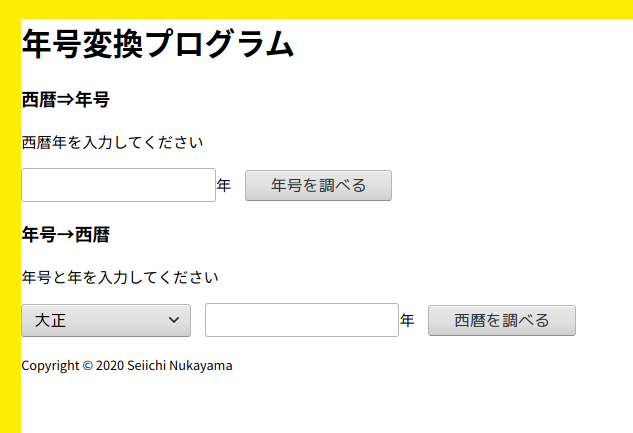
\includegraphics[width=10cm]{gamen01.png}

このコードの特徴は、西暦から年号を求めるフォームと、年号から西暦を求めるフォームの2種類があることで、西暦から年号を求めるフォームは ''Xnengo''サーブレットに処理を渡しています。年号から西暦を求めるフォームは ''Xseireki''サーブレットに処理を渡しています。


\subsubsection{サーブレットを作成}

まず、''Xnengo''サーブレットを作成します。
これは、index.jspの ''年号を求める''ボタンを押すと、このサーブレットにデータが送られます。

プロジェクトの ''nengo'' を右クリックして、''新規'' - ''サーブレット'' を選択します。''サーブレット作成''ダイアログが開くので、以下のように入力します。

''ソース・フォルダー'' は、そのまま(/nengo/src)。

''Javaパッケージ'' は、「com.example.nengo」とします。

''クラス名''は、「Xnengo」とします。

''スーパークラス''は、そのままでいいです。(javax.servlet.http.HttpServlet)

「完了」をクリックすると、Xnengoサーブレットのひな型でひらきます。

今回は、POSTしか使いませんので、''doGet''メソッドは削除してください。

また、''doPost''メソッドの中の ''doGet(request, response)'' は、削除して
おいてください。

そして、''doPost''メソッドを以下のようにしてください。

\begin{lstlisting} [caption=Xnengo.java, numbers=none]
protected void doPost(HttpServletRequest request, HttpServletResponse
        response) throws ServletException, IOException {

    // JSPから受け取る文字列を UTF-8 とします。
    request.setCharacterEncoding("UTF-8");

    // index.jspにデータを送り返すのに、セッションという
    // しくみを使います。
    HttpSession session = request.getSession(true);    // --- <1>

    // index.jspから送られてきたデータ(seireki)を
    // 受け取って、txtSeirekiという文字列にセット。
    String txtSeireki = request.getParameter("seireki"); // --- <2>

    // index.jspからのデータが null あるいは 空 の場合
    if (txtSeireki != null && txtSeireki != "") {      
        this.toNengo(txtSeireki);                      // --- <3>
        session.setAttribute("nengo", this.nengo);     // --- <4>
        session.setAttribute("nen", this.nen)
        session.setAttribute("error", null);
        session.setAttribute("seireki", null);
    }
    else {
        session.setAttribute("nengo", null);           // --- <5>
        session.setAttribute("nen", null);
        session.setAttribute("seireki", null);
        session.setAttribute("error", this.ERROR);
    }
    response.sendRedirect("/nengo");                   // --- <6>
}
\end{lstlisting}

\begin{enumerate}
 \item \textgt{セッション変数}を使ってクライアント(index.jspをダウンロー
       ドしたユーザーのブラウザ)にデータを送ります。
 \item \textgt{post}で送られてきた \textgt{seireki} というラベルがつけら
       れたデータを取得。
 \item \textgt{Xnengo}クラスのメソッド \textgt{toNengo}に seirekiデータ
       を送り、クラス変数 this.nengo と this.nen に年号と年をセットしま
       す。このメソッドは後ほど作ります。
 \item セッション変数''nengo''に、this.nengo をセットします。このセッショ
       ン変数は、クライアントのブラウザに送られます。
 \item クライアントから post で seireki データが送られてこなかった場合、
       クライアントのブラウザに送るセッション変数には ``null''をセットし
       ます。これは、``''でもいいかもしれません。
 \item http://XXXXXXX/nengo というURLにアクセスするようにクライアントに
       指示します。       
\end{enumerate}


\subsubsection{index.jspでセッション変数を受け取る}

Xnengoサーブレットから、西暦データが \textgt{''seireki''}という名前でセッ
ションを使って送られてくるので、それを受け取るようにします。

\begin{lstlisting}[numbers=none]
    <%
    String sekireki = session.getAttribute(``seireki'');
    %>
\end{lstlisting}

もしも null ならば、``''データにします。

\begin{lstlisting}[numbers=none]
    <%
    if (seiseki == null) { seiseki = ``''; }
    %>
\end{lstlisting}

これを \verb!<body>! タグ内で表示するために文字列にします。

\begin{lstlisting}[numbers=none]
    String printSeireki = ``西暦'' + seireki + ``です。``;
\end{lstlisting}

これを \verb!<body>!タグ 内で、以下のようにして表示します。

\begin{lstlisting}[numbers=none]
    <%= printSeireki %>
\end{lstlisting}

ところで、Java8からは、Optional というやり方が使えるようになりました。

\begin{lstlisting}[numbers=none]
    Object objNengo = Optional.ofNullable(session.getAttribute("nengo")).orElse("");
    nengo = (String) objNengo;
\end{lstlisting}

Optional以下のメソッドで

\begin{tcolorbox}
ofNullbable() -- ()内の変数ないしメソッドが null を含むことを想定している。
    もし、null でなければ、その値が、objNengo にセットされる。

orElse(値) -- もし、nullであれば、()内の値にする。
\end{tcolorbox}

Optional は、Object型を返すので、次の行では、それを String型にキャストしてます。

\textgt{index.jsp}は、以下のようになります。


\begin{lstlisting} [caption=index.jsp]
<%@ page language="java" contentType="text/html; charset=UTF-8"
         pageEncoding="UTF-8" %>
<%@ page import="javax.servlet.http.*"
         import="java.util.*"
         import="java.io.IOException" %>

<%
String error = "a";
String ansNengo = "";
String ansSeireki = "";
String nengo = "";
String nen = "";
String seireki = "";

Object objNengo = Optional.ofNullable(session.getAttribute("nengo")).orElse("");
nengo = (String) objNengo;

Object objNen = Optional.ofNullable(session.getAttribute("nen")).orElse("");
nen = (String) objNen.toString();

Object objSeireki = Optional.ofNullable(session.getAttribute("seireki")).orElse("");
seireki = (String) objSeireki.toString();

Object objError = Optional.ofNullable(session.getAttribute("error")).orElse("");
error = (String) objError;


if (nengo != "" && nen != "" ) {
  ansNengo = nengo + " " + String.valueOf(nen) + " 年です";
}
if (seireki != "") {
  ansSeireki = "西暦 " + String.valueOf(seireki) + " 年です";
}

%>
<!doctype html>
<html lang="ja">
  <head>
    <meta charset="utf-8"/>
    <title>年号変換プログラム</title>
    <link rel="stylesheet" href="css/nengo.css"/>
  </head>
  <body>
    <div id="wrap">
      <header>
        <h1>年号変換プログラム</h1>
      </header>
      <article>
        <section>
          <h1>西暦⇒年号</h1>
          <form action="http://localhost:8080/nengo/xnengo" method="post">
            <p>西暦年を入力してください</p>
            <p><input type="text" name="seireki" id="seireki"/>年
              &nbsp;&nbsp;
              <input type="submit" value="年号を調べる"/></p>
          </form>
          <div id="kaito-nengo"><%= ansNengo %></div>
        </section>
        <section>
          <h1>年号→西暦</h1>
          <form action="http://localhost:8080/nengo/xseireki" method="post">
            <p>年号と年を入力してください</p>
            <p><select name="nengo" id="nengo">
              <option value="" selected>選択してください</option>
              <option value="明治">明治</option>
              <option value="大正">大正</option>
              <option value="昭和">昭和</option>
              <option value="平成">平成</option>
              <option value="令和">令和</option>
              <option value="未来">未来</option>
            </select>
            &nbsp;&nbsp;
            <input type="text" name="nen" id="nen"/>年
            &nbsp;&nbsp;
            <input type="submit" value="西暦を調べる"/></p>
          </form>
          <div id="kaito-seireki"><%= ansSeireki %></div>
        </section>
      </article>
      <footer>
        <small>Copyright &copy; 2020 Seiichi Nukayama</small>
        <p><%= error %></p>
      </footer>
    </div>
  </body>
</html>
\end{lstlisting}




\end{document}

%% 修正時刻: Sat May  2 15:10:04 2020


%% 修正時刻: Tue May 12 06:51:28 2020
